% BRACIS 2026 — Springer LNCS/LNAI format
% Double-blind submission — anonymized
%
\documentclass[runningheads]{llncs}
%
\usepackage[T1]{fontenc}
%
\usepackage{graphicx}
\usepackage{url}
\usepackage{subcaption}
\providecommand{\doi}[1]{\url{https://doi.org/#1}}
%
% URLs in blue roman font according to Springer's eBook style:
\usepackage{color}
\renewcommand\UrlFont{\color{blue}\rmfamily}
\urlstyle{rm}
%
\begin{document}
%
\title{Real-Time Fall Detection with CNN-LSTM: Video-Level\\Evaluation and Cross-Dataset Generalization via Fine-Tuning}
%
\titlerunning{CNN-LSTM Fall Detection: Cross-Dataset Generalization via Fine-Tuning}
%
\author{Anonymous Author(s)}
%
\authorrunning{Anonymous}
%
\institute{Anonymous Institution}
%
\maketitle
%
\begin{abstract}
Small, controlled fall-detection datasets routinely produce near-perfect benchmark scores that collapse when the model meets a new environment. We investigate this generalization gap using a MobileNetV2+LSTM architecture trained on the UR Fall Detection Dataset (URFD) under a \textbf{video-level split} (GroupShuffleSplit) to prevent temporal data leakage. As expected, all variants --- CNN-LSTM, CNN-only, frozen backbone, and ablations --- reach 100\% accuracy on URFD, confirming the dataset's performance ceiling. Cross-dataset evaluation on the \textbf{Le2i Fall Detection Dataset} (191~clips, four environments) then separates the approaches: the fine-tuned model achieves \textbf{97.07\% accuracy with zero missed falls} (FN=0), while the identical architecture with a frozen backbone misses 11~falls at 96.16\% accuracy --- a clinically relevant difference of roughly one missed fall in thirteen. These results show that \textbf{fine-tuning is necessary, not optional}, for cross-environment generalization. Beyond the model, we integrate a full alert pipeline: classification on a PC, local alarm via ESP32, and push notification through a React Native application, all connected by MQTT, with a temporal confirmation mechanism (threshold 75\%, 3~consecutive predictions) to reduce false positives in deployment.

\keywords{Fall detection \and CNN-LSTM \and Transfer learning \and Cross-dataset evaluation \and Fine-tuning \and Computer vision \and IoT}
\end{abstract}
%
%
%
\section{Introduction}

Every year, at least one third of adults over 65 fall at least once~\cite{lord2001,heinrich2010}. The injury itself is often less harmful than the time spent on the floor: an elderly person who falls and cannot get up alone faces substantially higher mortality and risk of long-term sequelae~\cite{kwolek2014}. Automating fall detection addresses precisely this window --- alerting caregivers before prolonged immobility causes secondary damage.

Existing approaches split into wearable-based (accelerometers and gyroscopes) and camera-based. Wearable systems work when the device is worn, but compliance is a persistent problem, and high-acceleration daily activities generate frequent false alarms~\cite{kwolek2014,mubashir2013}. RGB cameras are non-intrusive but sensitive to lighting and lack depth cues~\cite{kwolek2014}. Hybrid methods combine both at the cost of added infrastructure.

Convolutional neural networks changed what is achievable with RGB video alone: CNNs extract spatial features without hand-crafted descriptors, and LSTM layers~\cite{lstm1997} can model the temporal trajectory of a movement --- the slump, the impact, the stillness --- rather than treating each frame in isolation~\cite{lu2019}. We took this as a starting point and built a complete system around it.

Rather than stopping at the model, we implemented the full alert chain: video capture and real-time classification on a PC, local alarm via an ESP32 microcontroller, and remote push notification through a React Native mobile application, all connected by MQTT. The contributions are:

\begin{enumerate}
  \item Development and validation of a hybrid CNN (MobileNetV2) + LSTM model for binary fall classification in video sequences, evaluated under a \textbf{video-level split} that prevents temporal data leakage;
  \item A quantitative comparison against two representative baselines (CNN-only without LSTM; CNN-LSTM without fine-tuning) and an ablation study isolating the contributions of fine-tuning, data augmentation, and LSTM capacity;
  \item \textbf{Cross-dataset validation} on the Le2i Fall Detection Dataset, demonstrating that fine-tuning achieves 100\% sensitivity (zero missed falls) across environments, while the frozen backbone misses 11 falls --- a clinically relevant difference;
  \item Implementation of a complete data pipeline (ETL) for the URFD and Le2i datasets, with sliding window extraction and data augmentation;
  \item Integration of a distributed alert system using MQTT, ESP32, and a mobile application, with a temporal confirmation mechanism to reduce false positives in real-time inference.
\end{enumerate}

\section{Related Work}

Kwolek and Kepski~\cite{kwolek2014} combined a triaxial accelerometer with Kinect depth maps, using a threshold on total acceleration ($SV > 3g$) followed by an SVM classifier, achieving 98.33\% accuracy and 100\% sensitivity on URFD. Sucerquia et al.~\cite{sisfall2017} presented SisFall and showed that threshold-based algorithms trained on young adults degrade significantly when applied to elderly subjects. Mubashir et al.~\cite{mubashir2013} surveyed fall detection approaches, noting that vision-based systems are non-intrusive but face challenges with lighting and occlusion. Lu et al.~\cite{lu2019} proposed 3D-CNN+LSTM for fall detection from video, demonstrating that temporal modeling is essential to distinguish falls from abrupt non-fall movements. Chhetri et al.~\cite{chhetri2021} further confirmed this using enhanced optical flow with deep learning. More recently, Alanazi et al.~\cite{alanazi2022} proposed a four-stream 3D-CNN (4S-3DCNN) architecture that fuses multi-level spatio-temporal features and achieved 100\% accuracy on URFD and Le2i simultaneously; and Chakraborty et al.~\cite{chakraborty2024} demonstrated 99.9\%+ detection by fusing audio (MobileNetV2 on Mel spectrograms) with video-based pose estimation on the Le2i dataset, highlighting the practical deployment potential of lightweight backbones for this task.

A recurring concern in the literature is the gap between reported benchmark performance and real-world generalization~\cite{thakkar2024}. Many studies use window-level or subject-dependent splits that inflate metrics through data leakage~\cite{lu2019,chhetri2021}. Patel et al.~\cite{patel2024} showed that fine-tuned transfer learning models achieve 98.15\% accuracy with explainability guarantees, and explicitly note that evaluation protocol choices substantially affect reported results.

Our work departs from this body of literature in several ways. We deliberately chose a backbone that runs on an ordinary CPU without a GPU, quantified the contribution of each design decision through controlled baselines and ablations rather than reporting a single model, adopted a video-level split that prevents the temporal leakage we found in common experimental setups, and went beyond model evaluation to deliver a working IoT system with embedded hardware and a mobile application.

\section{Methodology}

\subsection{Dataset and Data Preparation}

We used the UR Fall Detection Dataset~\cite{kwolek2014} from the University of Rzesz\'{o}w (Poland): 30~fall sequences and 40~normal daily activity (ADL) sequences captured by RGB cameras. The dataset also provides depth maps and accelerometer readings, but we restricted ourselves to the RGB channel to evaluate a purely visual approach on accessible hardware.

\subsubsection{Preprocessing Pipeline (ETL).}
The extraction, transformation, and loading pipeline performs the following steps:
\begin{enumerate}
  \item \textbf{Recursive scan:} automatic identification of image files in heterogeneous subdirectories;
  \item \textbf{Media conversion:} transformation of PNG image sequences into AVI videos at 30\,fps using OpenCV;
  \item \textbf{Resizing:} normalization of all frames to $128 \times 128$ pixels;
  \item \textbf{Intensity normalization:} scaling to $[0, 1]$ applied on-the-fly in the \texttt{tf.data} pipeline (frames are stored as \texttt{uint8} to reduce memory footprint by a factor of~4);
  \item \textbf{Sliding window:} extraction of subsequences of $T = 20$~frames with stride of 10, generating multiple samples per video;
  \item \textbf{Video-level split:} \textit{GroupShuffleSplit} with 80/20 ratio grouping by video identifier, ensuring that no window from a test video appears in training.
\end{enumerate}

The pipeline yielded \textbf{1,111~samples} (850~Normal, 261~Fall), each with dimensions $(20, 128, 128, 3)$, distributed across 56~training videos and 14~test videos. Fig.~\ref{fig:pipeline} illustrates the complete data pipeline.

\begin{figure}
\centering
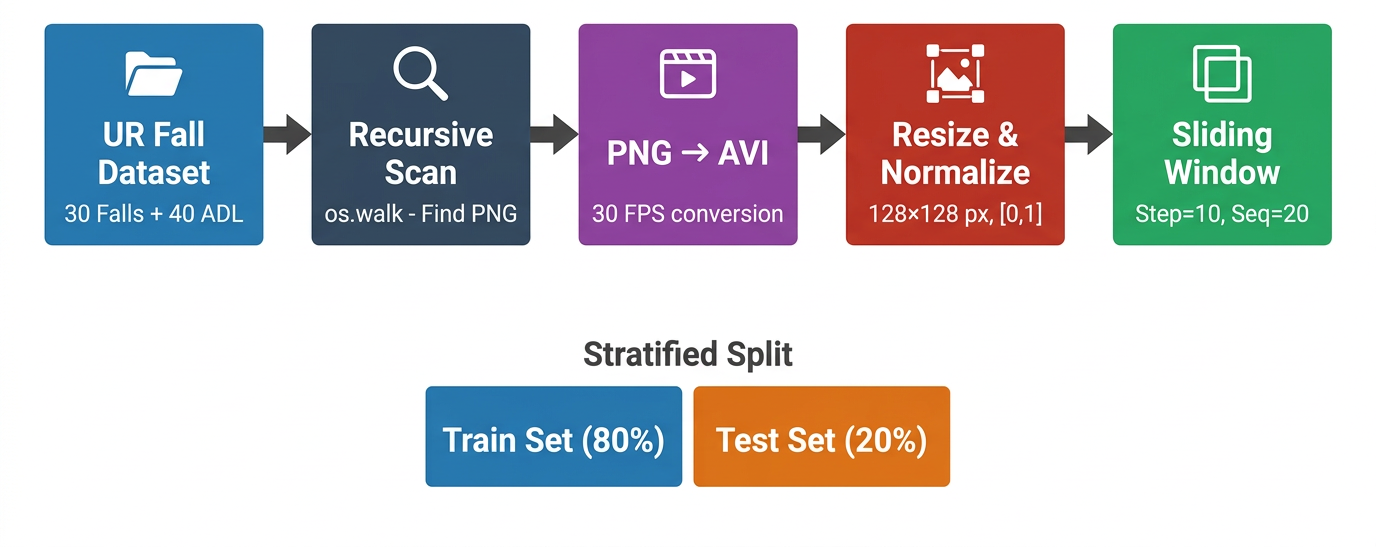
\includegraphics[width=0.88\textwidth]{pipeline_dados_branco.png}
\caption{Data preprocessing pipeline (ETL).}\label{fig:pipeline}
\end{figure}

\subsubsection{Video-Level Split.}
A random window-level split can place windows from the same video on both sides of the train/test boundary. Under stride 10, adjacent windows share up to 18 of their 20 frames, so the model effectively memorizes test data. We use \textbf{GroupShuffleSplit} with the video identifier as the group key, ensuring that all windows from a given video land entirely in training or entirely in the test set. This is the conservative choice and arguably the only one that reflects real deployment, where the model will face completely new recording sessions.

\subsubsection{Data Augmentation.}
At training time we apply random horizontal flips (50\% probability) and brightness variation ($\pm 20\%$). Both transforms are applied identically to every frame in the window so the temporal structure is not disturbed. Whether augmentation actually helps is tested in the ablation (Section~\ref{sec:ablation}).

\subsection{Model Architecture}

The architecture has three stages (Fig.~\ref{fig:arquitetura}): a CNN that processes each frame independently, an LSTM that reads the resulting sequence, and a dense classifier with dropout.

\begin{figure}
\centering
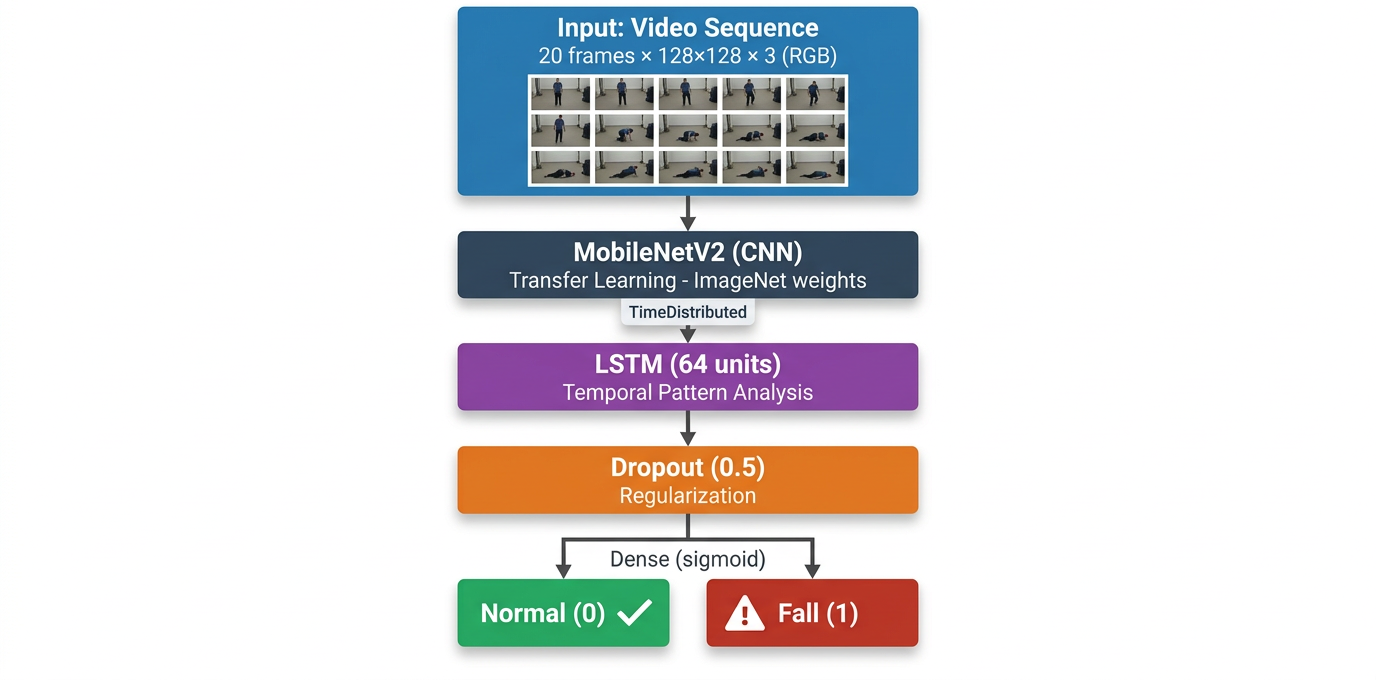
\includegraphics[width=0.82\textwidth]{arquitetura_modelo_cnn_lstm_branco.png}
\caption{Architecture of the proposed hybrid CNN+LSTM model.}\label{fig:arquitetura}
\end{figure}

\subsubsection{Spatial Feature Extractor --- MobileNetV2.}
We chose MobileNetV2~\cite{mobilenetv2} for its inverted-residual depthwise-separable architecture, which keeps parameter count low enough for CPU inference. Pre-trained ImageNet weights provide a strong starting point~\cite{patel2024}; we then unfreeze the last 30 layers for fine-tuning, which we later show is necessary for cross-environment robustness~\cite{patel2024,chakraborty2024}. A \textbf{TimeDistributed} wrapper applies the same CNN to each of the $T = 20$~frames, producing a 1,280-dimensional feature vector per frame for the LSTM to consume.

\subsubsection{Temporal Analysis --- LSTM.}
An LSTM layer~\cite{lstm1997} with 64~units receives the feature vector sequence and captures how movement evolves over the 20-frame window. The gating mechanisms (input, forget, output) selectively retain what matters and discard noise, which is useful for a task where the signal of interest (the moment of a fall) spans only a fraction of the sequence.

\subsubsection{Classification and Regularization.}
The LSTM output is regularized by \textbf{Dropout} (rate 0.5) and fed to a \textbf{Dense} layer with a single neuron and \textbf{sigmoid} activation, producing the fall probability $p \in [0,1]$.

\subsection{Baselines and Ablation Study}\label{sec:baselines}

We trained six variants under identical hyperparameters. The \textbf{full CNN-LSTM} is the main model: fine-tuning of the last 30 MobileNetV2 layers, augmentation on, LSTM with 64 units. Two baselines test specific components: \textbf{CNN-only} replaces the LSTM with GlobalAveragePooling1D (does temporal modeling matter?) and \textbf{CNN-LSTM frozen} keeps the entire backbone frozen (does fine-tuning matter?). Three ablations then switch off fine-tuning, augmentation, or increase LSTM capacity to 128 units one at a time.

\subsection{Training}

Table~\ref{tab:hyperparams} summarizes the training hyperparameters (identical across all variants to ensure fair comparison).

\begin{table}
\centering
\caption{Training hyperparameters.}\label{tab:hyperparams}
\begin{tabular}{|l|l|}
\hline
\textbf{Parameter} & \textbf{Value} \\
\hline
Optimizer & Adam \\
Initial learning rate & $1 \times 10^{-4}$ \\
Loss function & Binary crossentropy \\
Batch size & 4 \\
Maximum epochs & 30 \\
Sequence length ($T$) & 20 frames \\
Input resolution & $128 \times 128$ pixels \\
Unfrozen layers (fine-tuning) & 30 \\
Dropout rate & 0.5 \\
\hline
\end{tabular}
\end{table}

Data loading used \texttt{tf.data.Dataset} with prefetch and shuffle. Training used three callbacks: \textbf{ModelCheckpoint} to save the best \texttt{val\_accuracy} checkpoint, \textbf{EarlyStopping} with patience 7 on \texttt{val\_loss}, and \textbf{ReduceLROnPlateau} that halves the learning rate after 3 stagnant epochs.

\subsubsection{Evaluation Metrics.}
Because the dataset is imbalanced and missing a fall carries a much higher cost than a false alarm, accuracy alone is insufficient. We report AUC-ROC, per-class precision and recall (sensitivity for the fall class, specificity for the normal class), F1-score, and the confusion matrix. Metrics are computed with \texttt{scikit-learn}.

\subsection{Real-Time Inference Optimizations}

Running the model in real time on an Intel i7 CPU with no GPU required several practical adjustments: calling \texttt{model(input, training=False)} directly instead of \texttt{model.predict()} to avoid per-call graph overhead; using a \texttt{deque} as a circular frame buffer; predicting every 5~frames (cutting CPU load by roughly 80\%); exporting to TFLite (2.4~MB); and working at $128\times128$ rather than the standard $224\times224$. False positives from quick movements (sitting down, bending) were addressed with a \textbf{temporal confirmation} rule: the alert fires only after $N=3$ consecutive predictions above $\theta=0.75$. Predictions between 0.5 and 0.75 show a ``Possible fall'' indicator without triggering the alarm.

\subsection{Integrated Alert System}

The alert system distributes notifications through the \textbf{MQTT} (Message Queuing Telemetry Transport) protocol~\cite{mqtt}, using the \textbf{Eclipse Mosquitto}~\cite{mosquitto} broker as a central message hub, as illustrated in Fig.~\ref{fig:sistema}.

\begin{figure}
\centering
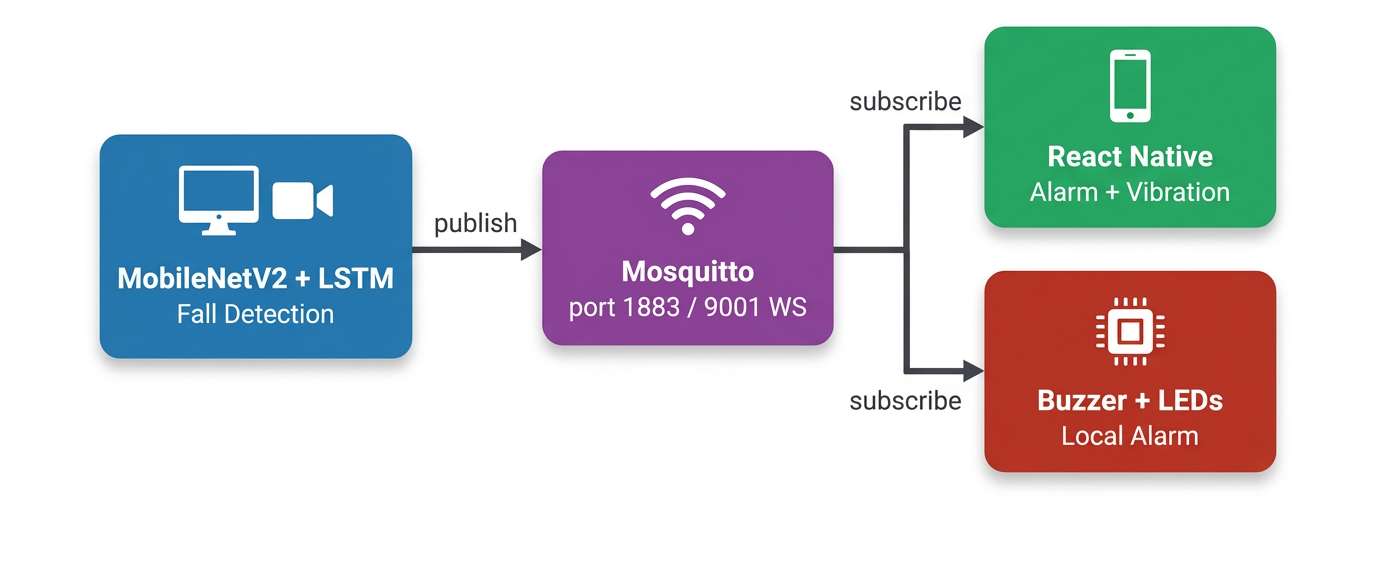
\includegraphics[width=0.88\textwidth]{arquitetura_sistema_branco.png}
\caption{Distributed alert system architecture.}\label{fig:sistema}
\end{figure}

Alert messages are transmitted in JSON format containing the fields: \texttt{alert} (event type), \texttt{confidence} (model confidence), \texttt{timestamp}, and \texttt{metadata} (frame ID, model name).

\subsubsection{Hardware Layer --- ESP32.}
The ESP32 microcontroller runs Arduino-based firmware that: receives alerts via Serial (USB, for testing) or MQTT (WiFi, for production); activates a passive buzzer (GPIO~18) and red LED (GPIO~19) for 10~seconds upon fall detection; and maintains a green LED (GPIO~21) as a system status indicator.

\subsubsection{Mobile Layer --- React Native Application.}
The application was developed with React Native (v0.81), Expo SDK~54, and TypeScript, connecting to the Mosquitto broker via WebSocket (port~9001). The four main screens are: (i)~\textbf{Dashboard} with MQTT connection status and alert statistics; (ii)~\textbf{Alarm} with automatic activation, looping audio, vibration, and ``Confirm Fall'', ``False Alarm'', and ``Call Emergency'' buttons; (iii)~\textbf{History} with persisted event log and category filters; and (iv)~\textbf{Settings} for broker address, confidence threshold, and emergency number. The software architecture uses Context API with \texttt{useReducer} for global state, and three decoupled services: MqttService, AlarmService, and EventStorage (AsyncStorage).

\section{Results}\label{sec:results}

\subsection{URFD Performance}\label{sec:urfd-results}

The video-level split (GroupShuffleSplit 80/20) yielded 861~training and 250~test samples across 56 and 14~videos, respectively (850~Normal, 261~Fall total). The full CNN-LSTM model achieved \textbf{100\% accuracy}, \textbf{1.0000 AUC-ROC}, and perfect precision, recall, and F1-score on both classes (218~TN, 32~TP, 0~FP, 0~FN; loss $3.93\times10^{-4}$). Figs.~\ref{fig:confusao}--\ref{fig:roc} present the confusion matrix and ROC curve.

\begin{figure}[h]
\centering
\begin{minipage}{0.46\textwidth}
  \centering
  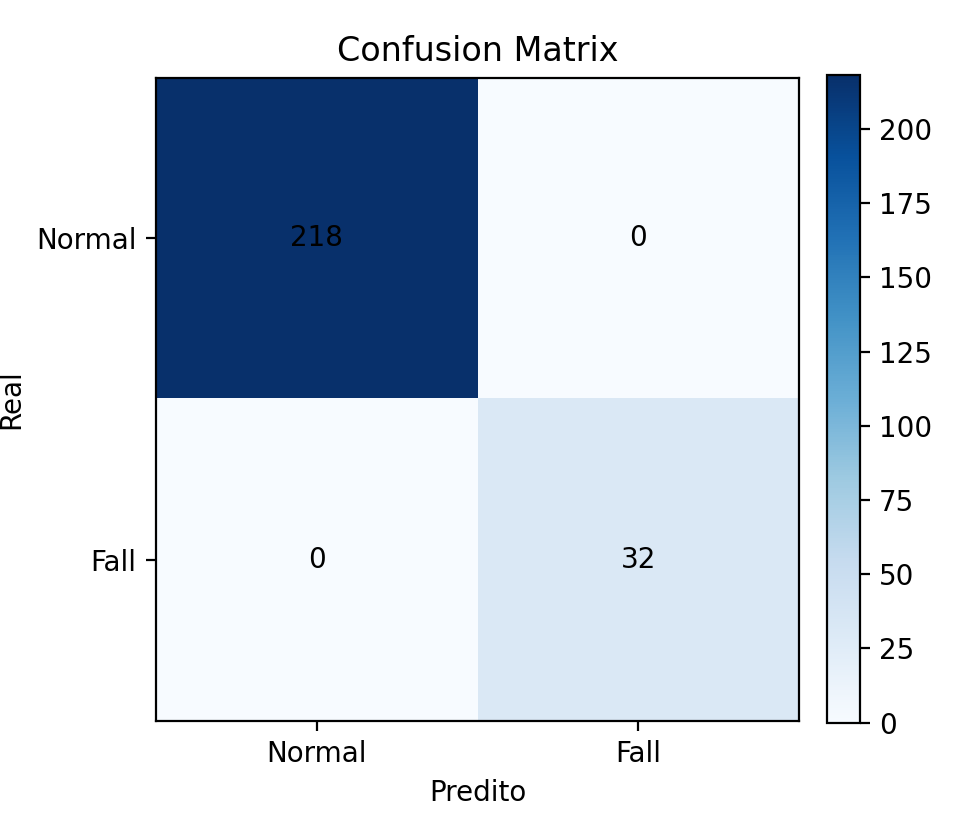
\includegraphics[width=\textwidth]{confusion_matrix.png}
  \caption{Confusion matrix --- URFD (218~TN, 32~TP, 0~FP, 0~FN).}\label{fig:confusao}
\end{minipage}\hfill
\begin{minipage}{0.46\textwidth}
  \centering
  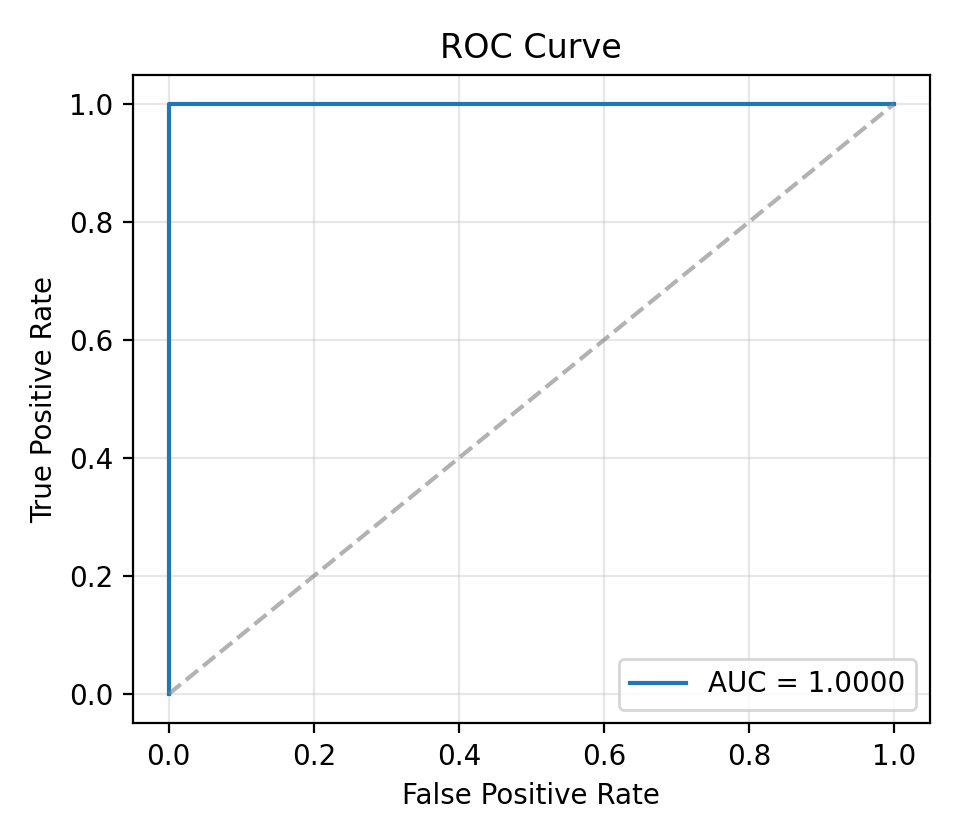
\includegraphics[width=\textwidth]{roc_curve.png}
  \caption{ROC curve --- URFD (AUC = 1.0000).}\label{fig:roc}
\end{minipage}
\end{figure}

\subsection{Baseline Comparison}\label{sec:baseline-results}

Table~\ref{tab:baselines} compares the full CNN-LSTM model against the CNN-only and CNN-LSTM frozen baselines. All variants share the same hyperparameters, video-level split, and random seed.

\begin{table}
\centering
\caption{Comparison against baselines on the held-out test set. Best results in \textbf{bold}.}\label{tab:baselines}
\begin{tabular}{|l|c|c|c|c|c|}
\hline
\textbf{Model} & \textbf{Acc.} & \textbf{AUC} & \textbf{Recall (Fall)} & \textbf{Prec. (Fall)} & \textbf{F1 (Fall)} \\
\hline
CNN-only (no LSTM)       & 100.00\% & 1.0000 & 1.0000 & 1.0000 & 1.0000 \\
CNN-LSTM (frozen)        & 100.00\% & 1.0000 & 1.0000 & 1.0000 & 1.0000 \\
\textbf{CNN-LSTM (full)} & \textbf{100.00\%} & \textbf{1.0000} & \textbf{1.0000} & \textbf{1.0000} & \textbf{1.0000} \\
\hline
\end{tabular}
\end{table}

\noindent All three variants achieve perfect scores on the URFD test set. This saturation indicates a \emph{performance ceiling}: the URFD dataset (70 videos, controlled laboratory environment) is not complex enough to discriminate between architectures. Cross-dataset validation on Le2i (Section~\ref{sec:le2i}) breaks this ceiling and reveals the contribution of fine-tuning.

\subsection{Ablation Study}\label{sec:ablation}

Table~\ref{tab:ablation} presents the ablation study, isolating the effect of fine-tuning, data augmentation, and LSTM capacity.

\begin{table}
\centering
\caption{Ablation study on the full CNN-LSTM model.}\label{tab:ablation}
\begin{tabular}{|l|c|c|c|c|c|}
\hline
\textbf{Variant} & \textbf{Acc.} & \textbf{AUC} & \textbf{Recall (Fall)} & \textbf{Prec. (Fall)} & \textbf{F1 (Fall)} \\
\hline
Full model (reference)  & \textbf{100.00\%} & \textbf{1.0000} & \textbf{1.0000} & \textbf{1.0000} & \textbf{1.0000} \\
--- no fine-tuning      & 100.00\% & 1.0000 & 1.0000 & 1.0000 & 1.0000 \\
--- no augmentation     & 100.00\% & 1.0000 & 1.0000 & 1.0000 & 1.0000 \\
--- LSTM 128 units      & 100.00\% & 1.0000 & 1.0000 & 1.0000 & 1.0000 \\
\hline
\end{tabular}
\end{table}

\noindent All ablations produce identical perfect scores on URFD, confirming the performance ceiling. Because URFD saturates all variants, it cannot discriminate between architectural choices. The differentiating experiment is the cross-dataset evaluation reported in Section~\ref{sec:le2i}, where removing fine-tuning causes 11~additional missed falls.

\subsection{Cross-Dataset Validation on Le2i}\label{sec:le2i}

Since all URFD variants hit 100\%, we needed a harder test. We retrained the three main variants on the \textbf{Le2i Fall Detection Dataset}~\cite{charfi2013}, which has 130~annotated videos across four different indoor environments (two coffee rooms and two homes). Le2i is still actively used in recent benchmarks~\cite{alanazi2022,chakraborty2024}, so results on it are comparable to the literature. The same pipeline applied: sliding window ($T=20$, stride~10), video-level split (80/20), $128\times128$ frames. Each annotated video was split into a Normal clip (frames before the fall, with a 5-frame margin) and a Fall clip (from fall onset onward), yielding 191~clips, 2,575~samples total, and a test set of \textbf{443~samples} (291~Normal, 152~Fall).

\begin{table}
\centering
\caption{Cross-dataset results on Le2i (443 test samples). Bold marks best per column.}\label{tab:le2i}
\begin{tabular}{|l|c|c|c|c|c|c|}
\hline
\textbf{Model} & \textbf{Acc.} & \textbf{AUC} & \textbf{Recall (Fall)} & \textbf{Prec. (Fall)} & \textbf{F1 (Fall)} & \textbf{FN} \\
\hline
CNN-only (no LSTM)        & \textbf{97.07\%} & \textbf{0.9888} & \textbf{1.0000} & \textbf{0.9212} & \textbf{0.9590} & \textbf{0} \\
\textbf{CNN-LSTM (full)}  & \textbf{97.07\%} & 0.9868 & \textbf{1.0000} & \textbf{0.9212} & \textbf{0.9590} & \textbf{0} \\
CNN-LSTM (frozen)         & 96.16\% & 0.9833 & 0.9276 & 0.9592 & 0.9431 & 11 \\
\hline
\end{tabular}
\end{table}

\begin{figure}[h]
\centering
\begin{minipage}{0.46\textwidth}
  \centering
  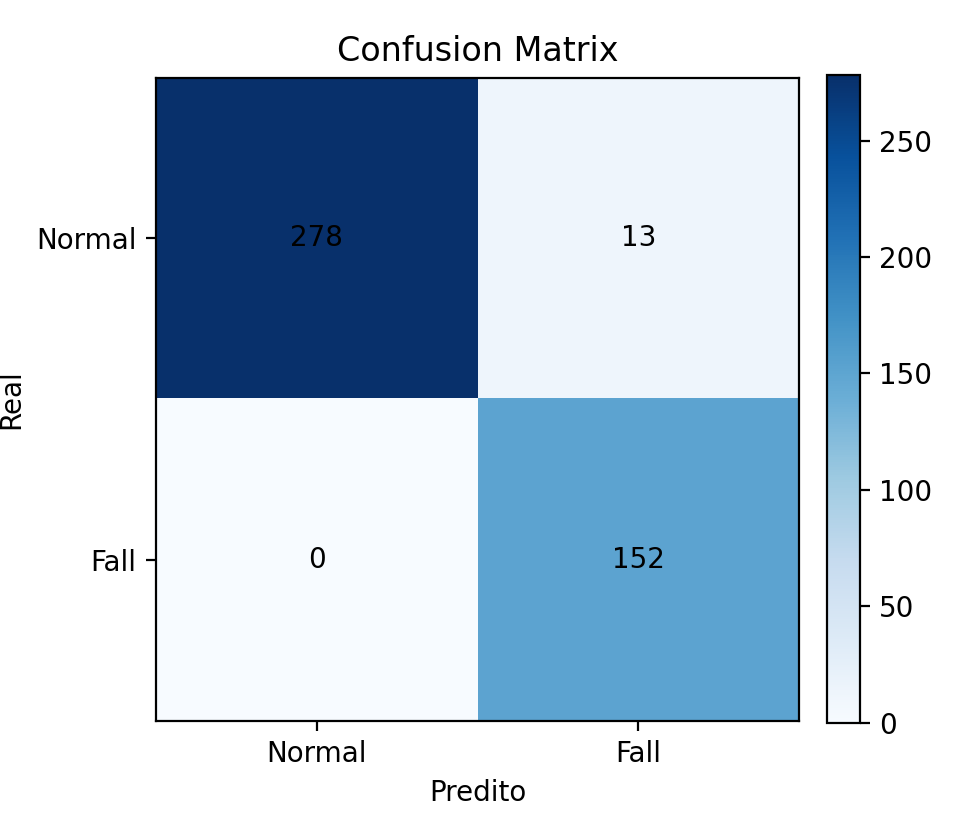
\includegraphics[width=\textwidth]{confusion_matrix_le2i.png}
  \caption{Confusion matrix --- Le2i (278~TN, 13~FP, 0~FN, 152~TP).}\label{fig:confusion_le2i}
\end{minipage}\hfill
\begin{minipage}{0.46\textwidth}
  \centering
  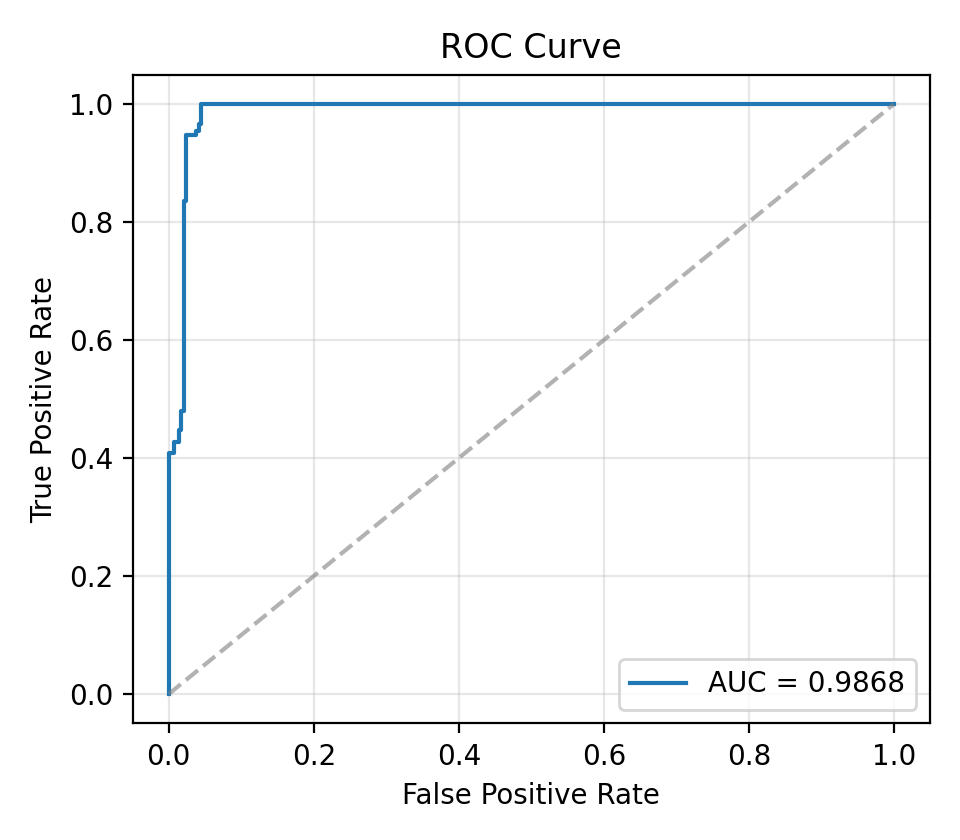
\includegraphics[width=\textwidth]{roc_curve_le2i.png}
  \caption{ROC curve --- Le2i (AUC = 0.9868).}\label{fig:roc_le2i}
\end{minipage}
\end{figure}

The main finding is in the FN column: frozen backbone misses 11 falls that both fine-tuned models catch. With a fine-tuned backbone, neither the CNN-only nor the CNN-LSTM variant produces any false negatives. That the two fine-tuned variants perform identically suggests the LSTM is not adding anything once the spatial features are well-adapted. Le2i fall clips appear to provide enough per-frame visual evidence after fine-tuning that temporal context becomes redundant. In a real deployment this distinction matters less than the gap versus the frozen model, where 11 undetected falls in 443 test samples translates to roughly one missed event per 40 windows.

\subsection{System Integration}

Integration tests via MQTT confirmed: messages from the Python module were received simultaneously by the ESP32 and the mobile application; the app triggered audio alarm, vibration, and automatic navigation to the alert screen; reconnection after simulated disconnections worked correctly; and event history persisted via AsyncStorage. On an Intel i7 CPU (8\,GB RAM), the temporal confirmation mechanism ($\theta=0.75$, $N=3$) eliminated premature detections, and frame skipping (every 5~frames) enabled smooth execution.

\section{Discussion}

\subsection{Analysis of Results}

Getting 100\% on URFD is not as strong a result as it sounds. The dataset has 70 videos recorded by a small number of participants in a controlled laboratory, always against a plain background. With a video-level split we still get perfect scores, which tells us the model learned something real, but it also tells us the data is not hard enough to expose differences between models. Sucerquia et al.~\cite{sisfall2017} showed a similar ceiling effect: algorithms that look near-perfect on controlled data can degrade substantially when the recording conditions or participant demographics change. Our cross-validation on Le2i (Section~\ref{sec:le2i}) was motivated by exactly this concern.

\subsubsection{On the Video-Level Split.}
Studies on URFD routinely report near-perfect metrics~\cite{lu2019,chhetri2021,alanazi2022}, and our results are no exception. We suspect part of this is genuine: MobileNetV2 features are rich enough that even a controlled dataset like URFD can be learned well. But part of it is methodological: window-level splits, which are common in the literature, place nearly identical frames on both sides of the train/test boundary. Thakkar et al.~\cite{thakkar2024} documented the same overestimation pattern in HAR benchmarks when subject-independent evaluation is skipped. Our numbers should be read as a lower bound, not an upper one: the model would likely perform better under a window-level split, but that is not the number that matters for deployment.

\subsection{Comparison with Related Work}

Table~\ref{tab:comparison} compares the results of the present work with approaches from the literature on the URFD dataset.

\begin{table}
\centering
\caption{Comparison with related work. URFD and Le2i use different inputs and splits; direct comparison is indicative only.}\label{tab:comparison}
\begin{tabular}{|l|l|c|c|c|c|}
\hline
\textbf{Work} & \textbf{Method / Dataset} & \textbf{Acc.} & \textbf{Sens.} & \textbf{Spec.} & \textbf{FN} \\
\hline
\cite{kwolek2014} & SVM + depth + accel. (URFD) & 98.33\% & 100\% & 96.67\% & 0 \\
\cite{kwolek2014} & Threshold UFT (URFD) & 95.00\% & 100\% & 90.00\% & 0 \\
\cite{charfi2013}  & Background subtraction (Le2i) & $\sim$95\% & $\sim$93\% & $\sim$97\% & -- \\
\cite{sisfall2017} & Threshold C8 (SisFall) & 96.10\% & 95.54\% & 96.38\% & -- \\
\textbf{This work} & \textbf{CNN-LSTM (URFD, video split)} & \textbf{100.00\%} & \textbf{100\%} & \textbf{100\%} & \textbf{0} \\
\textbf{This work} & \textbf{CNN-LSTM (Le2i, video split)} & \textbf{97.07\%} & \textbf{100\%} & 95.53\% & \textbf{0} \\
\hline
\end{tabular}
\end{table}

Numbers across rows of Table~\ref{tab:comparison} are not directly comparable: Kwolek and Kepski used depth maps and accelerometers, while we used RGB only; split strategies and cohort sizes also differ. We include the table to provide context, not to claim superiority over methods with access to richer sensor data. What we can say is that on the Le2i benchmark, where Charfi et al.~\cite{charfi2013} originally reported around 93\% sensitivity, our fine-tuned model reaches 100\% sensitivity with no missed falls, using only an RGB camera and a standard laptop CPU.

\subsubsection{On Fine-Tuning and Cross-Dataset Generalization.}
Le2i is where the experiments become informative. On URFD every variant saturates, so there is nothing to learn from comparing them. On Le2i, the frozen backbone misses 11 falls that the fine-tuned models do not. Eleven missed falls in a 443-sample test is not a statistical artifact: it means a system deployed without fine-tuning would fail to detect roughly one in thirteen falls in this environment. We interpret this as ImageNet features being insufficiently specific to the visual characteristics of fall events in varied indoor settings. Fine-tuning adapts the last 30 layers of MobileNetV2 to what distinguishes a falling person from someone sitting down quickly or bending over, and that adaptation appears necessary for cross-environment robustness.

\subsection{Limitations and Future Work}

The two datasets used are both staged: volunteers perform falls in a controlled setting. Whether the model transfers to genuine, unscripted falls in homes with different cameras and backgrounds is unknown. Datasets like OmniFall~\cite{sigurdsson2025}, which includes over 15k in-the-wild recordings, would be a demanding next test. Elderly participants in particular are underrepresented; as Sucerquia et al.~\cite{sisfall2017} showed, young-adult training data does not transfer cleanly to older subjects.

Camera use in domestic settings raises privacy concerns that local inference (the model already runs on CPU) and no-storage policies help address, but do not fully resolve. The 2.4~MB TFLite model is small enough for Raspberry Pi or similar edge hardware~\cite{guo2025}, which would remove the PC requirement entirely. On the application side, background push notifications are not yet implemented, meaning a caregiver who closes the app would miss an alert.

\section{Conclusion}

We built a fall detection system from the model up to the caregiver notification: a MobileNetV2+LSTM classifier running on a standard laptop, a local ESP32 alarm, and a React Native mobile app, all wired together over MQTT. On URFD, every variant we tested reached 100\% accuracy under a video-level split, which confirmed the model works but also exposed the limits of a single small benchmark. On Le2i, the picture became more interesting: fine-tuned models achieved 97.07\% accuracy with zero missed falls, while the frozen backbone missed 11. That gap is the most concrete finding of this work. Fine-tuning is not optional if the model needs to transfer across environments.

The TFLite export (2.4~MB) and frame-skipping inference ran smoothly on an i7 CPU with no GPU. The temporal confirmation mechanism ($\theta = 0.75$, $N = 3$) handled the false-positive problem at deployment time without retraining.

What remains is the harder part: validation with real elderly participants in domestic environments, a privacy-preserving edge deployment, and evaluation on larger, messier datasets such as OmniFall~\cite{sigurdsson2025}. The current results are a solid foundation for that work.

\begin{credits}
\subsubsection{\ackname}
This study was supported by a scientific initiation (PAIC) program. Details are omitted for double-blind review compliance. The Le2i dataset was obtained via Kaggle (tuyenldvn/falldataset-imvia). Parts of this manuscript were drafted with the assistance of a large language model (Claude, Anthropic); all content, results, and conclusions are the sole responsibility of the authors.

\subsubsection{\discintname}
The authors have no competing interests to declare that are relevant to the content of this article.
\end{credits}
%
% ---- Bibliography ----
%
% \bibliographystyle{splncs04}
% \bibliography{mybibliography}
%
\begin{thebibliography}{12}

\bibitem{alanazi2022}
Alanazi, T., Muhammad, G.: Human fall detection using 3D multi-stream convolutional neural networks with fusion. Diagnostics \textbf{12}(12), 3060 (2022). \doi{10.3390/diagnostics12123060}

\bibitem{chakraborty2024}
Chakraborty, S., Das, B., Roy, A.: Multimodal fall detection for solitary individuals based on audio-video decision fusion processing. Heliyon \textbf{10}(9), e28895 (2024). \doi{10.1016/j.heliyon.2024.e28895}

\bibitem{charfi2013}
Charfi, I., Miteran, J., Dubois, J., Atri, M., Tourki, R.: Optimized spatio-temporal descriptors for real-time fall detection: comparison of SVM and Adaboost-based classification. Journal of Electronic Imaging \textbf{22}(4), 041106 (2013)

\bibitem{chhetri2021}
Chhetri, S., Alsadoon, A., Al-Dala'in, T., Prasad, P.W.C., Rashid, T.A., Maag, A.: Deep learning for vision-based fall detection system: enhanced optical dynamic flow. arXiv preprint arXiv:2104.05744 (2021)

\bibitem{heinrich2010}
Heinrich, S., Rapp, K., Rissmann, U., Becker, C., K\"{o}nig, H.-H.: Cost of falls in old age: a systematic review. Osteoporosis International \textbf{21}, 891--902 (2010)

\bibitem{igual2013}
Igual, R., Medrano, C., Plaza, I.: Challenges, issues and trends in fall detection systems. BioMedical Engineering OnLine \textbf{12}(1), 1--24 (2013)

\bibitem{lstm1997}
Hochreiter, S., Schmidhuber, J.: Long Short-Term Memory. Neural Computation \textbf{9}(8), 1735--1780 (1997)

\bibitem{kwolek2014}
Kwolek, B., Kepski, M.: Human fall detection on embedded platform using depth maps and wireless accelerometer. Computer Methods and Programs in Biomedicine \textbf{117}(3), 489--501 (2014)

\bibitem{lord2001}
Lord, S., Sherrington, C., Menz, H.: Falls in Older People: Risk Factors and Strategies for Prevention. Cambridge University Press, Cambridge (2001)

\bibitem{lu2019}
Lu, N., Wu, Y., Feng, L., Song, J.: Deep learning for fall detection: three-dimensional CNN combined with LSTM on video kinematic data. IEEE Journal of Biomedical and Health Informatics \textbf{23}(1), 314--323 (2019)

\bibitem{mobilenetv2}
Sandler, M., Howard, A., Zhu, M., Zhmoginov, A., Chen, L.-C.: MobileNetV2: inverted residuals and linear bottlenecks. In: Proc. IEEE/CVF Conference on Computer Vision and Pattern Recognition (CVPR), pp. 4510--4520 (2018)

\bibitem{guo2025}
Guo, H., Tang, X., Park, K.: MicroFallNet: a lightweight model for real-time fall detection on smart wristbands. Biomedical Signal Processing and Control \textbf{86}, 105520 (2025). \doi{10.1016/j.bspc.2025.105520}

\bibitem{mosquitto}
Eclipse Foundation: Eclipse Mosquitto -- an open source MQTT broker, \url{https://mosquitto.org/}, last accessed 2026/03/23

\bibitem{mqtt}
OASIS: MQTT Version 3.1.1 -- OASIS Standard, \url{https://mqtt.org/}, last accessed 2026/03/23

\bibitem{mubashir2013}
Mubashir, M., Shao, L., Seed, L.: A survey on fall detection: principles and approaches. Neurocomputing \textbf{100}, 144--152 (2013)

\bibitem{patel2024}
Patel, A.N., Murugan, R., Maddikunta, P.K.R., Yenduri, G., Jhaveri, R.H., Gadekallu, T.R.: AI-powered trustable and explainable fall detection system using transfer learning. Image and Vision Computing \textbf{150}, 105164 (2024). \doi{10.1016/j.imavis.2024.105164}

\bibitem{sigurdsson2025}
Sigurdsson, G.A., et al.: OmniFall: from staged through synthetic to wild, a unified multi-domain dataset for robust fall detection. arXiv preprint arXiv:2505.19889 (2025)

\bibitem{sisfall2017}
Sucerquia, A., L\'{o}pez, J.D., Vargas-Bonilla, J.F.: SisFall: a fall and movement dataset. Sensors \textbf{17}(1), 198 (2017)

\bibitem{thakkar2024}
Thakkar, A., Trivedi, D., Bhatt, V.: A feature engineering method for smartphone-based fall detection. Sensors \textbf{25}(20), 6500 (2025). \doi{10.3390/s25206500}

\end{thebibliography}
\end{document}
